% arara: indent: {overwrite: yes}
\section{Лабораторная 3}

\subsection{Условие}

\textbf{Согласно варианту 10:}
\begin{enumerate}
	\item Нормальное $N(m, s^{2}), m = 1, s^{2} = 9$; Логонормальное $LN(m, s^{2}), m = 1, s^{2} = 9$; Экспоненциальное $E(\alpha), \alpha = 2$;
	\item Нормальное $N(m, s^{2}), m = 0, s^{2} = 1$; Лапласа $L(\alpha), \alpha = 0.5$; Вейбула $W(a, b), a = 1, b = 0.5$;
\end{enumerate}

Смоделировать непрерывную случайную величину. Исследовать точность моделирования.

\begin{enumerate}
	\item Осуществить моделирование $n = 1000$ реализаций СВ из нормального закона распределения $N(m, s^{2})$ с заданными параметрами. Вычислить несмещённые оценки математического ожидания и дисперсии, сравнить их с истинными;
	\item Смоделировать $n = 1000$ СВ из заданных абсолютно непрерывных распределений. Вычислить несмещённые оценки математического ожидания и дисперсии, сравнить их с истинными значениями (если это возможно);
	\item Для каждой из случайных величин построить свой критерий Колмогорова с уровнем значимости $\varepsilon = 0.05$. Проверить, что вероятность ошибки I рода стремится к 0.05;
	\item Для каждой из случайных величин построить свой $\chi^{2}$-критерий Пирсона с уровнем значимости $\varepsilon = 0.05$. Проверить, что вероятность ошибки I рода стремится к $0.05$;
	\item Осуществить проверку каждой из сгенерированных выборок каждым из построенных критериев.
\end{enumerate}

\subsection{Теория}
\subsubsection{Датчик случайной величины нормального распределения}

\textbf{Нормальное распределение} -  распределение вероятностей, которое в одномерном случае задаётся функцией плотности вероятности, совпадающей с функцией Гаусса.\\

\textbf{Функция распределения:}
\begin{equation}
	\frac{1}{2}(1+erf\left[\frac{x-\mu}{\sqrt{2\sigma^{2}}}\right].
\end{equation}

\textbf{Функция плотности:}
\begin{equation}
	\frac{1}{\sigma\sqrt{2\pi}} \cdot \exp\left[\frac{(x-\mu)^{2}}{2\sigma^{2}}\right].
\end{equation}

\textbf{Математическое ожидание:} $\mu$.\\

\textbf{Дисперсия:} $\sigma^{2}$.

\paragraph{Алгоритм моделирования:}\
\\

При моделировании будем использовать \textbf{преобразование Бокса-Мюллера}. Пусть $r$ b $\phi$ - независимые случайные величины, равномерно распределённые на интервале $(0, 1]$. Вычислим $z_{0}, z_{1}$ по формулам:

\begin{equation}
  \begin{array}{l}
	z_{0} = \cos(2\pi\phi)\sqrt{-2\ln(r)},\\
	z_{1} = \sin(2\pi\phi)\sqrt{-2\ln(r)}.
  \end{array}
\end{equation}

Тогда $z_{0}, z_{1}$ будут независимы и распределены нормально с математическим ожиданием 0 и дисперсией 1.

\subsubsection{Датчик случайной величины логнормального распределения}

\textbf{Логнормальное распределение} -  это двухпараметрическое семейство абсолютно непрерывных распределений. Если СВ имеет логнормальное распределение, то её логарифм имеет нормальное распределение.\\

\textbf{Функция распределения:}
\begin{equation}
	\frac{1}{2}+\frac{1}{2} Erf\left[\frac{\ln(x) - \mu}{\sigma\sqrt{2}}\right].
\end{equation}

\textbf{Функция плотности:}
\begin{equation}
	\exp\left[\frac{\left(\frac{\ln(x)-\mu}{\sigma}\right)^{2}}{2}\right]/\left(x\sigma\sqrt{2\pi}\right).
\end{equation}

\textbf{Математическое ожидание:} $e^{\mu+\sigma^{2}/2}$.\\

\textbf{Дисперсия:} $(e^{\sigma^{2}}-1)\cdot e^{2\mu+\sigma^{2}}$.

\paragraph{Алгоритм моделирования:}\
\\

Для моделирования обычно используется связь с нормальным распределением. Поэтому, достаточно сгенерировать нормально распределённую СВ, например, используя \textbf{преобразование Бокса-Мюллера}, и вычислить её экспонент.

\subsubsection{Датчик случайной величины экспоненциального распределения}

\textbf{Экспоненциальное распределение} - абсолютно непрерывное распределение, моделирующее время между двумя последовательными свершениями одного и того же события.\\

\textbf{Функция распределения:}
\begin{equation}
	1-e^{\lambda x}.
\end{equation}

\textbf{Функция плотности:}
\begin{equation}
	\lambda e^{-\lambda x}.
\end{equation}

\textbf{Математическое ожидание:}
\begin{equation}
	\lambda^{-1}.
\end{equation}

\textbf{Дисперсия:}
\begin{equation}
	\lambda^{-2}.
\end{equation}

\paragraph{Алгоритм моделирования:}\
\\

\begin{enumerate}
	\item Моделирование реализации $\alpha$ БСВ;
	\item Вычисление экспоненциально распределённой СВ:
	      \begin{equation}
		      x = -\frac{1}{\lambda}\ln(\alpha)
	      \end{equation}
\end{enumerate}

\subsubsection{Датчик случайной величины распределения Лапласа}

\textbf{Распределение Лапласа} - в теории вероятностей это непрерывное распределение случайной величины, при котором плотность вероятности есть $f(x)=\frac{\alpha}{2} \cdot e^{-\alpha|x-\beta|}, -\infty < x < +\infty$, где $\alpha > 0$ - параметр масштаба, $-\infty < \beta < +\infty$ - параметр сдвига.\\

\textbf{Функция распределения:}
\begin{equation}
	\begin{cases}{}
		\frac{1}{2}e^{\alpha(x-\beta)}\\
		1-\frac{1}{2}e^{\alpha(x-\beta)}
	\end{cases}.
\end{equation}

\textbf{Функция плотности:}
\begin{equation}
	\frac{\alpha}{2}e^{-\alpha|x-\beta|}.
\end{equation}

\textbf{Математическое ожидание:}
\begin{equation}
	\beta.
\end{equation}

\textbf{Дисперсия:}
\begin{equation}
	\frac{2}{\alpha^{2}}.
\end{equation}

\paragraph{Алгоритм моделирования:}\
\\
Алгоритм моделирования $\xi \thicksim L(\lambda)$ основан на методе обратной функции. Обратная для функции распределения $F_{\xi}(x)$ функция имеет вид:

\begin{equation}
	\begin{cases}
		x = F_{\xi}^{-1}(y) = \frac{1}{\lambda}\ln(2y) < 0, y \in [0, 0.5)\\
		x = F_{\xi}^{-1}(y) = \frac{1}{\lambda}\ln(2(1-y)) < 0, y \in [0.5, 1)
		\label{laplace_generator:ref}
	\end{cases}
\end{equation}

Для моделирования реализация $x$ СВ $\xi \thicksim L(\lambda)$ выполняются следующие действия:
\begin{enumerate}
	\item Моделирование реализации $\alpha$ БСВ;
	\item Принимается решение о том, что реализацией СВ $\xi$ является величина $x$, вычисляемая по формулам (\ref{laplace_generator:ref}) согласно отрезку, которому принадлежит $y$.
\end{enumerate}

\subsubsection{Датчик случайной величины распределения Вейбула}

\textbf{Распределение Вейбула} - в теории вероятностей это двухпараметрическое семейство абсолютно непрерывных распределений.\\

\textbf{Функция распределения:}
\begin{equation}
	1-e^{-(x/\lambda)^{k}}.
\end{equation}

\textbf{Функция плотности:}
\begin{equation}
	\frac{k}{\lambda} \cdot \left(\frac{x}{\lambda}\right)^{k-1} \cdot e^{-(x/\lambda)^{k}}.
\end{equation}

\textbf{Математическое ожидание:}
\begin{equation}
	\lambda\Gamma\left(1+\frac{1}{k}\right).
\end{equation}

\textbf{Дисперсия:}
\begin{equation}
	\lambda^{2}\Gamma\left(1+\frac{2}{k}\right) - \mu^{2}.
\end{equation}

\paragraph{Алгоритм моделирования:}\
\\
Алгоритм моделирования $\xi \thicksim WG(\lambda, k)$ основан на методе обратной функции. Обратная для функции распределения $F_{\xi}(x)$ функция имеет вид:

\begin{equation}
		x = F_{\xi}^{-1}(y) = \left(-\frac{1}{\lambda}\ln(y)\right)^{1/k}.
		\label{weibul_generator:ref}
\end{equation}

Для моделирования реализация $x$ СВ $\xi \thicksim L(\lambda)$ выполняются следующие действия:
\begin{enumerate}
	\item Моделирование реализации $\alpha$ БСВ;
	\item Принимается решение о том, что реализацией СВ $\xi$ является величина $x$, вычисляемая по формулам (\ref{weibul_generator:ref}), где $y=\alpha$.
\end{enumerate}

\subsection{Код программы}

\lstinputlisting[language=Python]{./lab_3/lab3.py}

\subsection{Результат выполнения}

\begin{figure}[H]
	\centering
	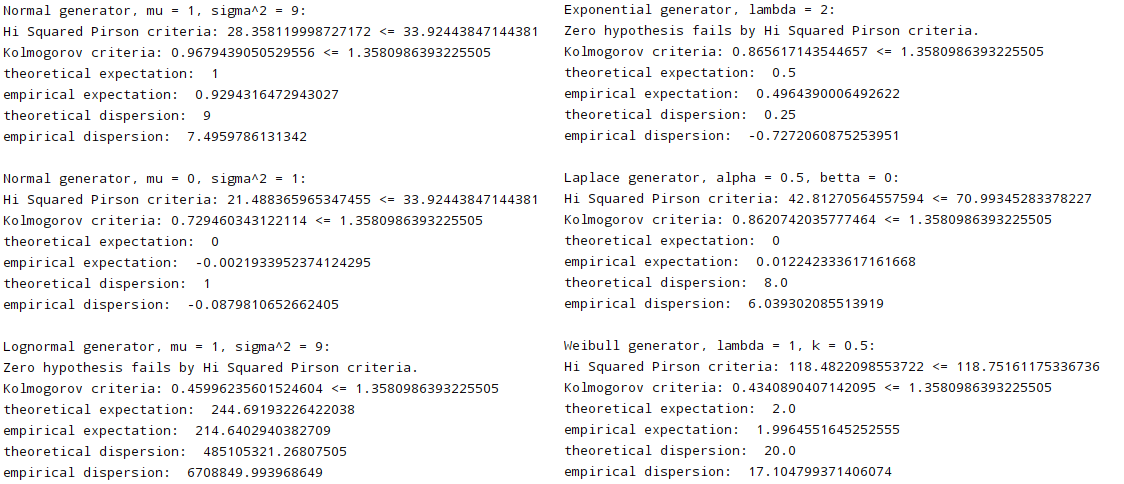
\includegraphics [width=\textwidth] {results_lab_3.png}
	\label{fig:results}
	\caption{Результат выполнения программы: проверка критерием согласия Пирсона и Колмогорова. Вывод теоретических и подсчёт эмпирических математических ожиданий и дисперсийё.}
\end{figure}

\begin{figure}[!h]
	\centering
	\begin{subfigure}[b]{0.45\textwidth}
		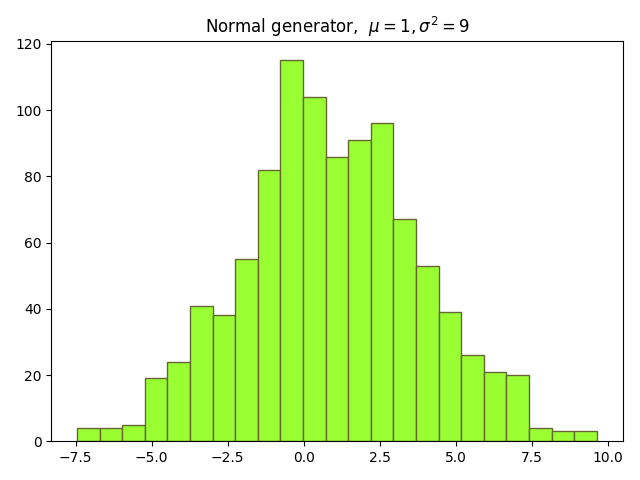
\includegraphics[width=\textwidth]{normal_generator_mu_1_sigma_3.png}
		\caption{Диаграмма выборки, полученной генератором нормального распределения при $\mu = 1, \sigma^{2} = 9$.}
	\end{subfigure}
	\hfill
	\begin{subfigure}[b]{0.45\textwidth}
		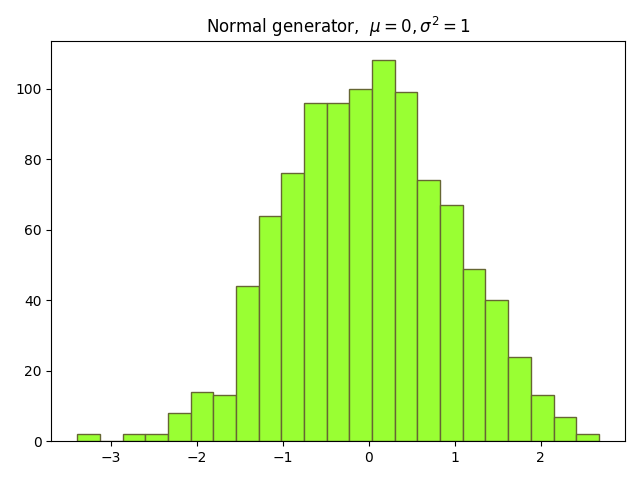
\includegraphics[width=\textwidth]{normal_generator_mu_0_sigma_1.png}
		\caption{Диаграмма выборки, полученной генератором нормального распределения при $\mu = 0, \sigma^{2} = 1$.}
	\end{subfigure}

\end{figure}
\begin{figure}[H]
	\centering
	\begin{subfigure}[b]{0.45\textwidth}
		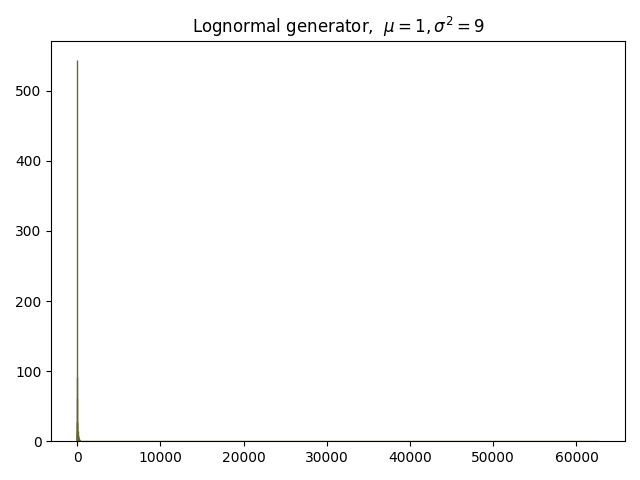
\includegraphics[width=\textwidth]{lognormal_generator_mu_1_sigma_3.png}
		\caption{Диаграмма выборки, полученной генератором логнормального распределения при $\mu = 1, \sigma^{2} = 9$.}
	\end{subfigure}
	\hfill
	\begin{subfigure}[b]{0.45\textwidth}
		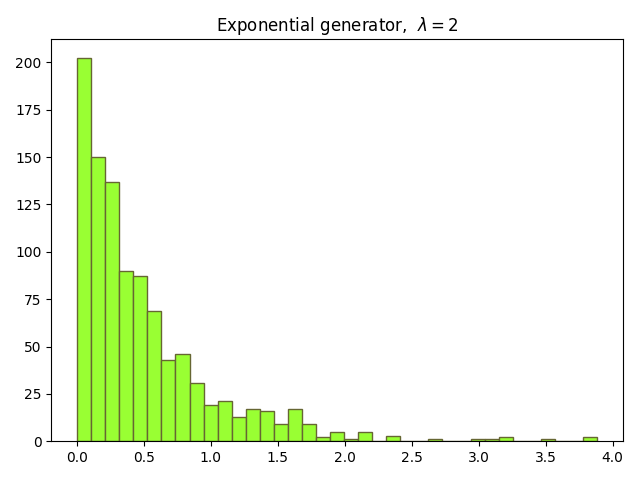
\includegraphics[width=\textwidth]{exponential_generator_lambda_2.png}
		\caption{Диаграмма выборки, полученной генератором экспоненциального распределения при $\lambda = 2$.}
	\end{subfigure}
	\\
	\begin{subfigure}[b]{0.45\textwidth}
		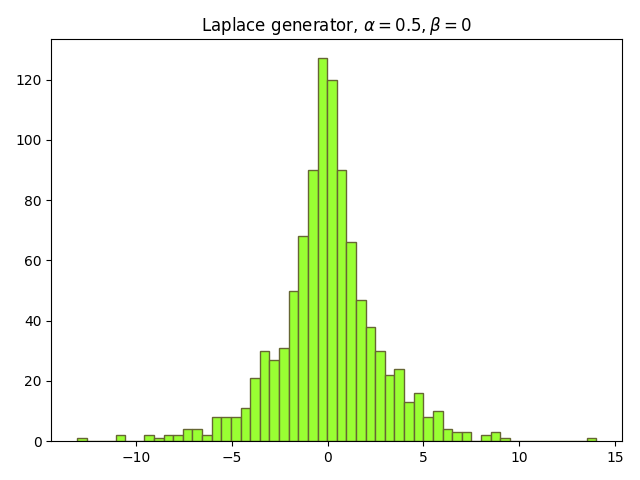
\includegraphics[width=\textwidth]{laplace_generator_alpha_0.5_betta_0.png}
		\caption{Диаграмма выборки, полученной генератором распределения Лапласа при $\alpha = 0.5, \beta = 0$.}
	\end{subfigure}
	\hfill
	\begin{subfigure}[b]{0.45\textwidth}
		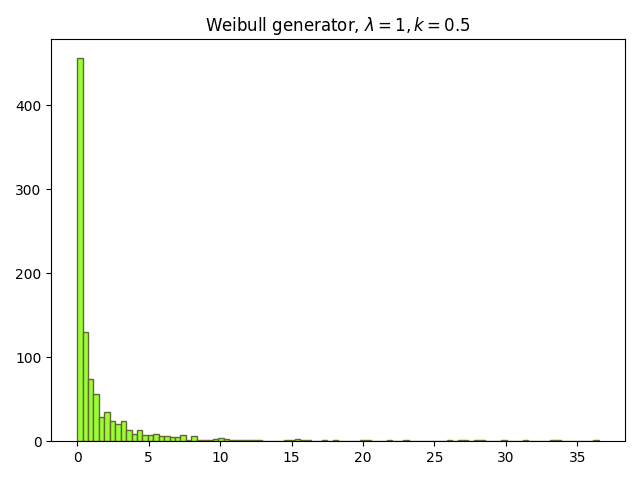
\includegraphics[width=\textwidth]{weibull_generator_lambda_1_k_0.5.png}
		\caption{Диаграмма выборки, полученной генератором распределения Вейбула при $\lambda = 1, k = 0.5$.}
	\end{subfigure}
\end{figure}
